\documentclass[border=3pt,tikz]{standalone}
% Shared look for every TikZ figure in these notes.
% Included by each standalone figure file; also keeps the figures consistent
% with the colours used in the PDF and on the website.

\usepackage{tikz}
\usepackage{pgfplots}
\pgfplotsset{compat=1.18}
\usetikzlibrary{arrows.meta, decorations.markings, decorations.pathmorphing,
                patterns, calc, positioning}
\usepackage{amsmath}

% Series colours are the three validated categorical slots also used by the
% interactive widgets, so a path drawn in the printed notes and the same path on
% the website are the same colour. They clear the colour-vision-deficiency and
% contrast checks as a set; every path is direct-labelled as well, so colour is
% never the only thing carrying identity.
\definecolor{duPurple}{HTML}{68246D}
\definecolor{duBlue}{HTML}{2A78D6}
\definecolor{duRed}{HTML}{EB6834}
\definecolor{duGreen}{HTML}{1BAF7A}
\definecolor{duGrey}{HTML}{6B6B6B}

\tikzset{
  axisline/.style   = {-{Stealth[length=3mm]}, line width=0.7pt, black},
  path1/.style      = {duBlue,   line width=1.1pt},
  path2/.style      = {duRed,    line width=1.1pt},
  path3/.style      = {duGreen,  line width=1.1pt},
  statedot/.style   = {circle, fill=black, inner sep=1.4pt},
  arrowhead/.style  = {decoration={markings,
                        mark=at position #1 with {\arrow{Stealth[length=2.6mm]}}},
                       postaction={decorate}},
  lbl/.style        = {font=\small},
  slbl/.style       = {font=\footnotesize, duGrey},
  workfill/.style   = {duPurple, opacity=0.16},
}

\begin{document}
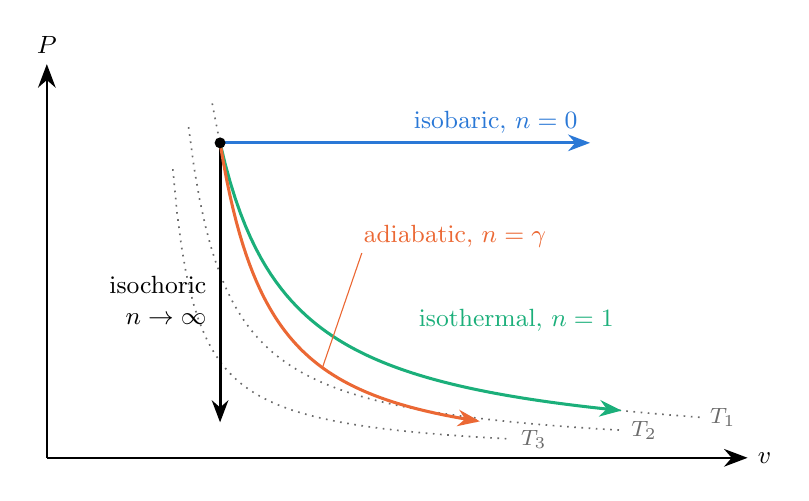
\begin{tikzpicture}
  \draw[axisline] (-1.3,0) -- (7.6,0) node[right, lbl] {$v$};
  \draw[axisline] (-1.3,0) -- (-1.3,5.0) node[above, lbl] {$P$};
  % dotted isotherms, T1 > T2 > T3
  \draw[duGrey, dotted, line width=0.6pt] plot[domain=0.8:7.0, samples=80] (\x, {3.6/\x});
  \node[slbl, right] at (7.0,{3.6/7.0}) {$T_1$};
  \draw[duGrey, dotted, line width=0.6pt] plot[domain=0.5:6.0, samples=80] (\x, {2.1/\x});
  \node[slbl, right] at (6.0,{2.1/6.0}) {$T_2$};
  \draw[duGrey, dotted, line width=0.6pt] plot[domain=0.3:4.6, samples=80] (\x, {1.1/\x});
  \node[slbl, right] at (4.6,{1.1/4.6}) {$T_3$};
  \coordinate (A) at (0.9,4.0);
  % isobaric n = 0
  \draw[duBlue, line width=1.1pt, -{Stealth[length=2.8mm]}] (A) -- (5.6,4.0);
  \node[lbl, duBlue, above] at (4.4,4.0) {isobaric, $n = 0$};
  % isochoric n -> infinity
  \draw[line width=1.1pt, -{Stealth[length=2.8mm]}] (A) -- (0.9,0.45);
  \node[lbl, left, align=right] at (0.85,2.0) {isochoric\\$n \to \infty$};
  % isothermal n = 1 (along T1)
  \draw[path3, -{Stealth[length=2.8mm]}] plot[domain=0.9:6.0, samples=80] (\x, {3.6/\x});
  \node[lbl, duGreen, anchor=west] at (3.3,1.75) {isothermal, $n = 1$};
  % adiabatic n = gamma: steeper, crosses to lower isotherms
  \draw[path2, -{Stealth[length=2.8mm]}] plot[domain=0.9:4.2, samples=80] (\x, {4.0*(0.9/\x)^1.4});
  \draw[duRed, line width=0.4pt] (2.2,{4.0*(0.9/2.2)^1.4}) -- (2.7,2.6);
  \node[lbl, duRed, anchor=south west] at (2.6,2.55) {adiabatic, $n = \gamma$};
  \node[statedot] at (A) {};
\end{tikzpicture}
\end{document}
